\chapter{Chapter 4 Supplemental Information}
\label{sec:app4}
\raggedbottom

\clearpage

\section{Supplemental Figures}


\begin{figure}[htbp]
\centering
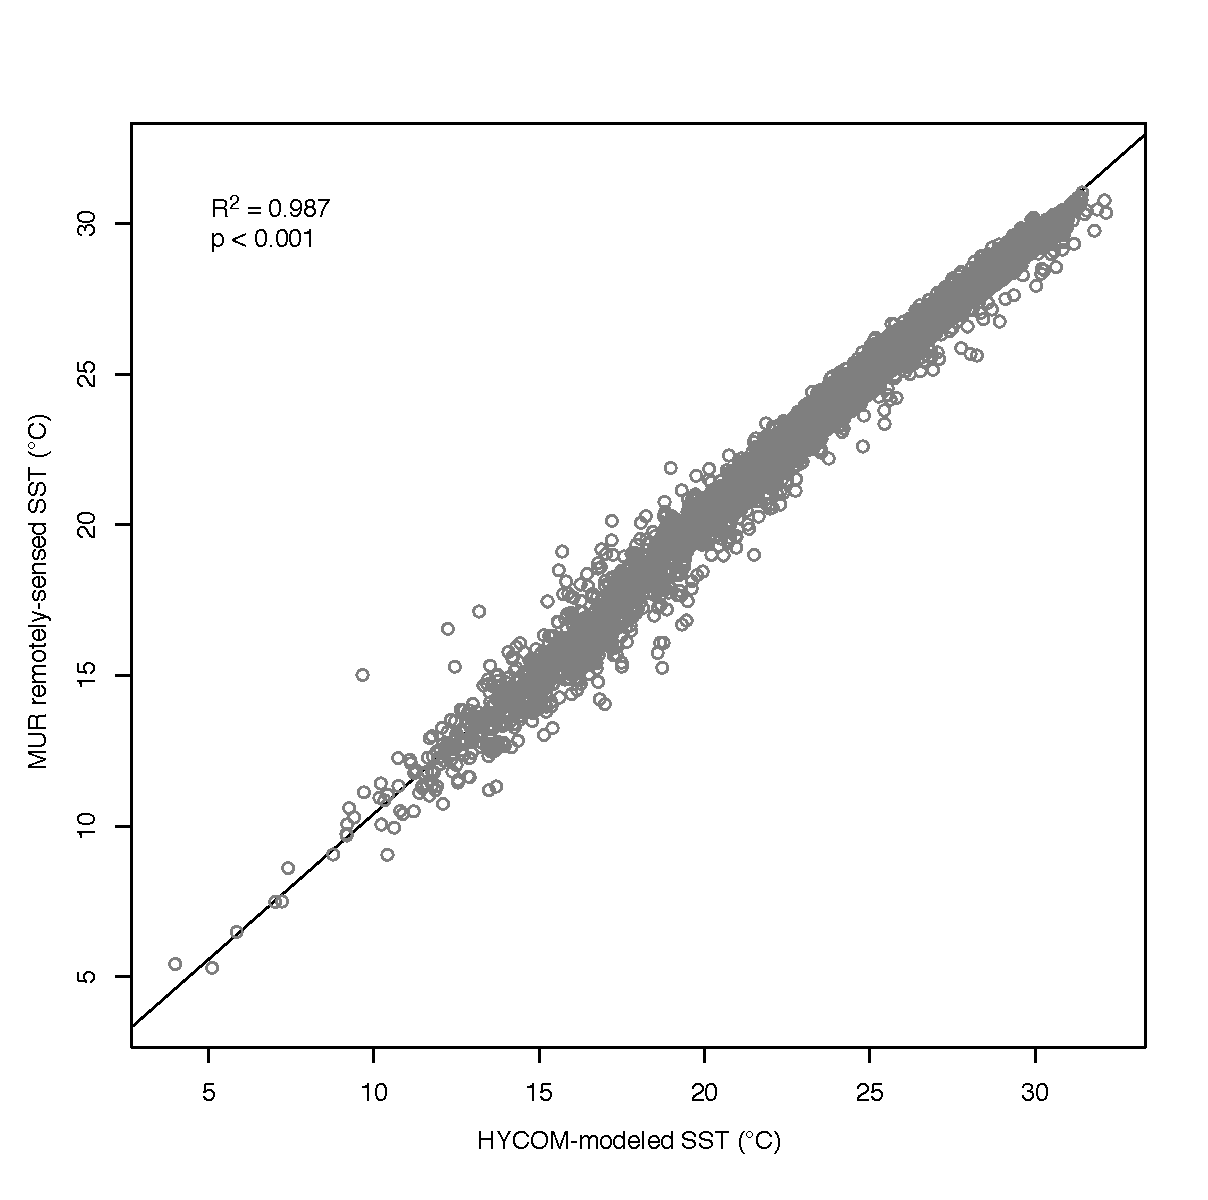
\includegraphics[width=\textwidth]{images/A4_FigS1.pdf}
\caption[Regression of remotely-sensed SST
and model-based SST at a subset of swordfish conventional tag
locations]{Regression of MUR remotely-sensed SST
and HYCOM (model-based) SST at a subset of swordfish conventional tag
locations.}
\label{fig:a4f1}
\end{figure}

\begin{figure}[htbp]
\centering
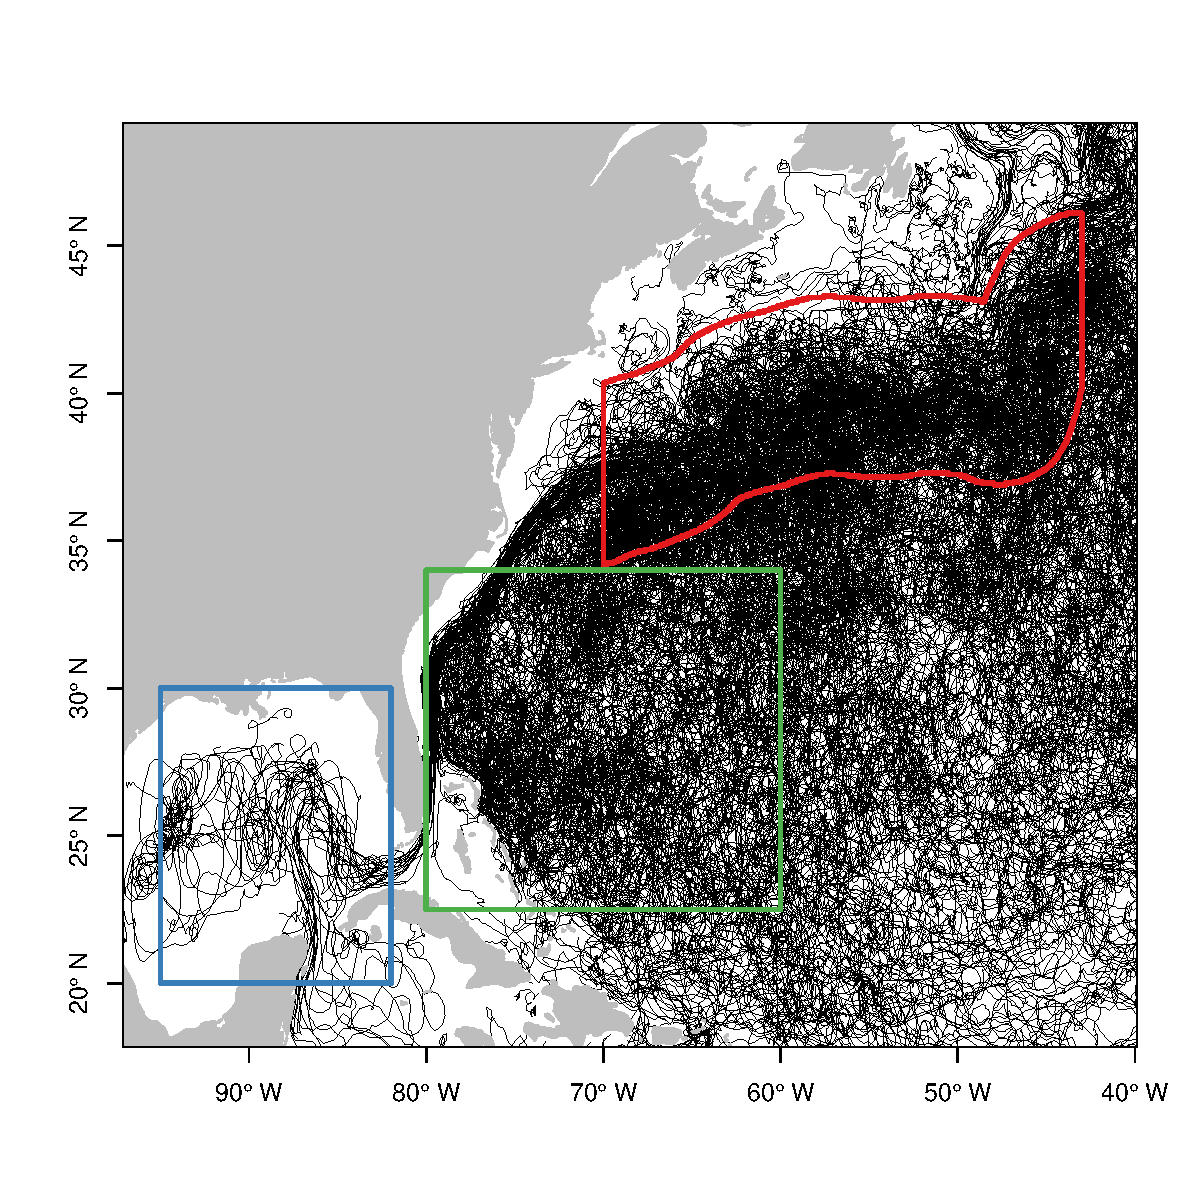
\includegraphics[width=\textwidth]{images/A4_FigS2.pdf}
\caption[Drifter trajectories used as null movements in the eddy collocation analysis]{Drifter trajectories used as null movements (black lines) and bounding boxes (colored lines) for the focal regions in the eddy collocation analysis. The data presented here has been trimmed to one location per day to aid visualization. Regions designate the Gulf Stream (red), Sargasso Sea (green) and Gulf of Mexico (blue).}
\label{fig:a4f2}
\end{figure}

\begin{figure}[htbp]
\centering
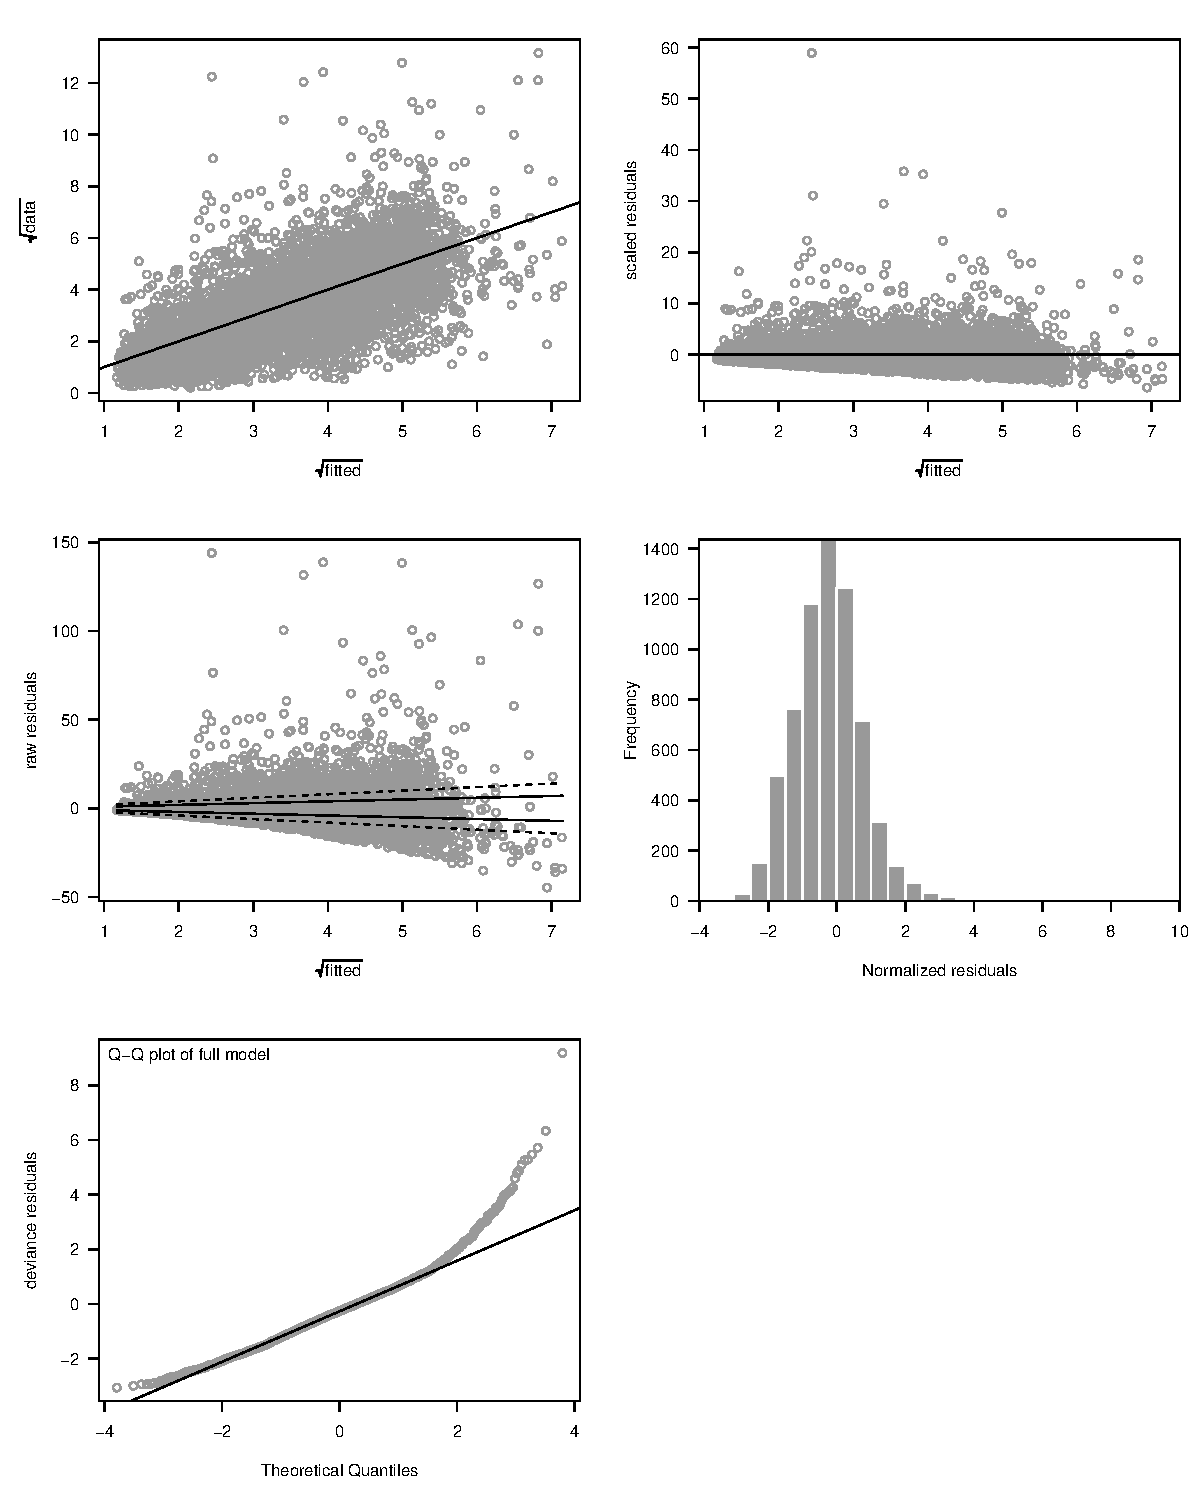
\includegraphics[width=\textwidth]{images/A4_FigS3.pdf}
\caption[Generalized additive model diagnostics for swordfish catch-per-unit effort]{Diagnostic plots for the final model
from the generalized additive model analysis of catch-per-unit effort
data. Code for generating these plots in \texttt{R} is from \citet{Lam2014}.}
\label{fig:a4f3}
\end{figure}

\begin{figure}[htbp]
\centering
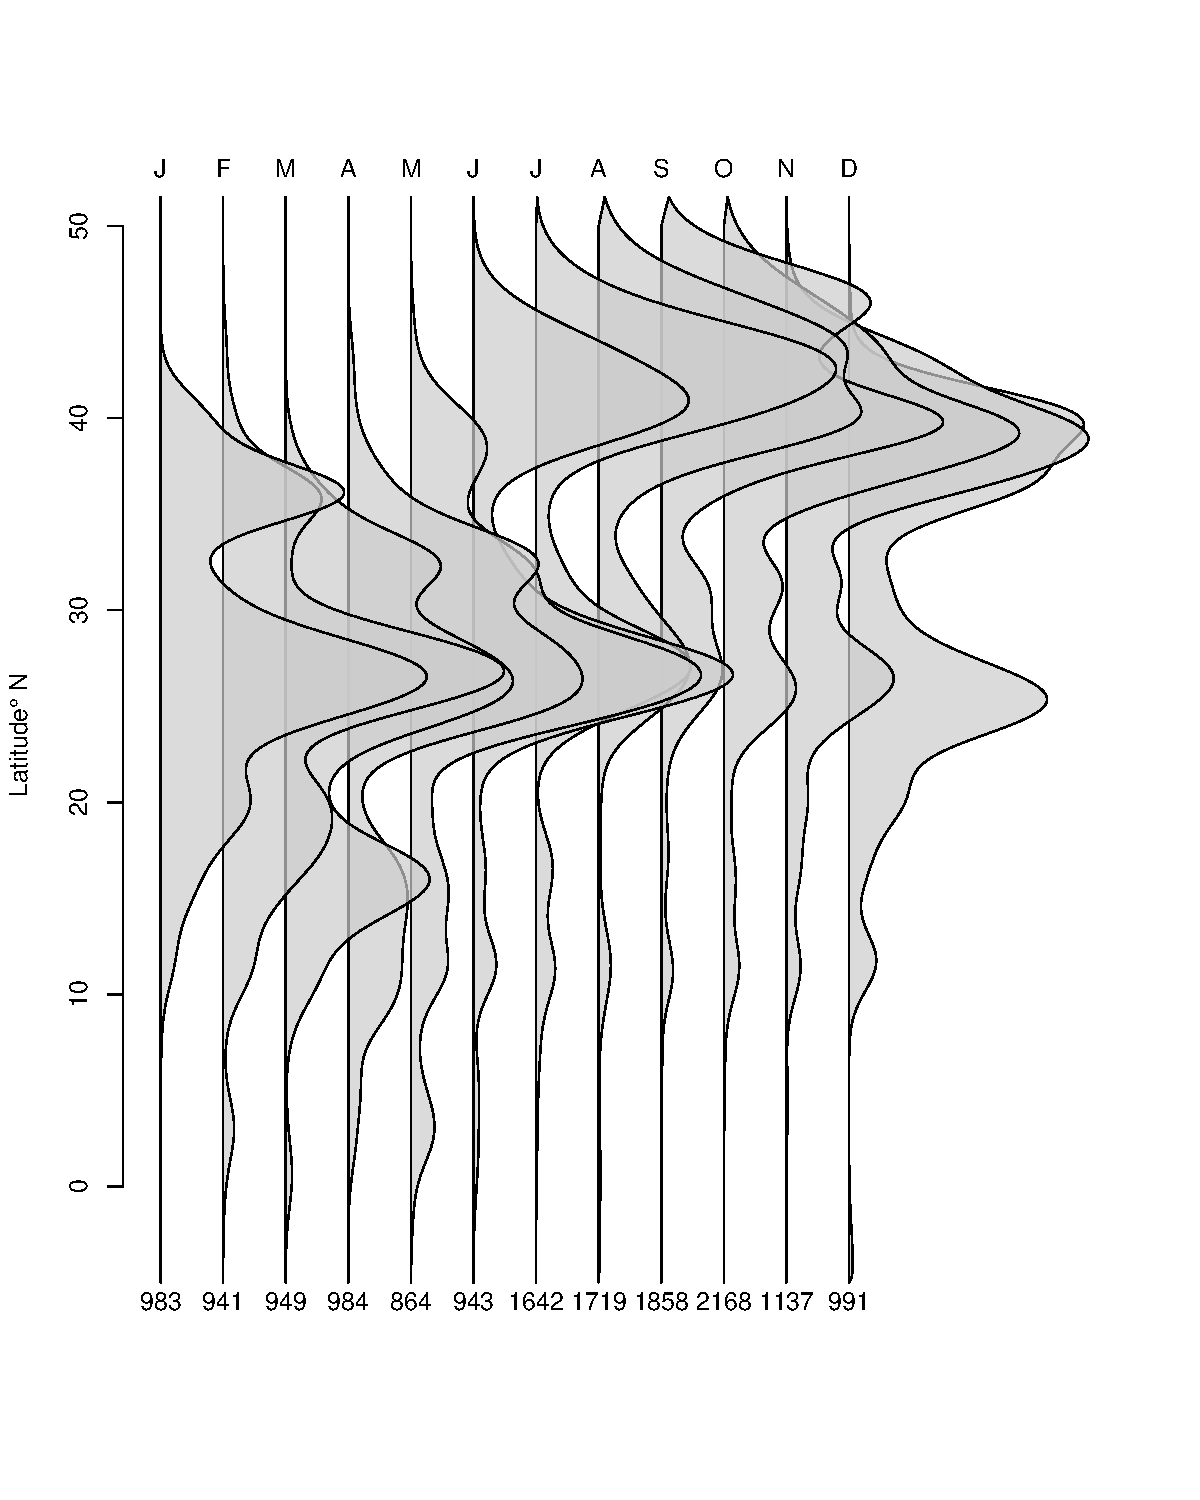
\includegraphics[width=\textwidth]{images/A4_FigS4.pdf}
\caption[Monthly latitude density distribution of
swordfish tagged with conventional tags]{Monthly density distribution of
swordfish tagged with conventional tags by latitude. Upper letters
indicate month and lower number labels indicate sample size of tagged
individuals.}
\label{fig:a4f4}
\end{figure}

\begin{figure}[htbp]
\centering
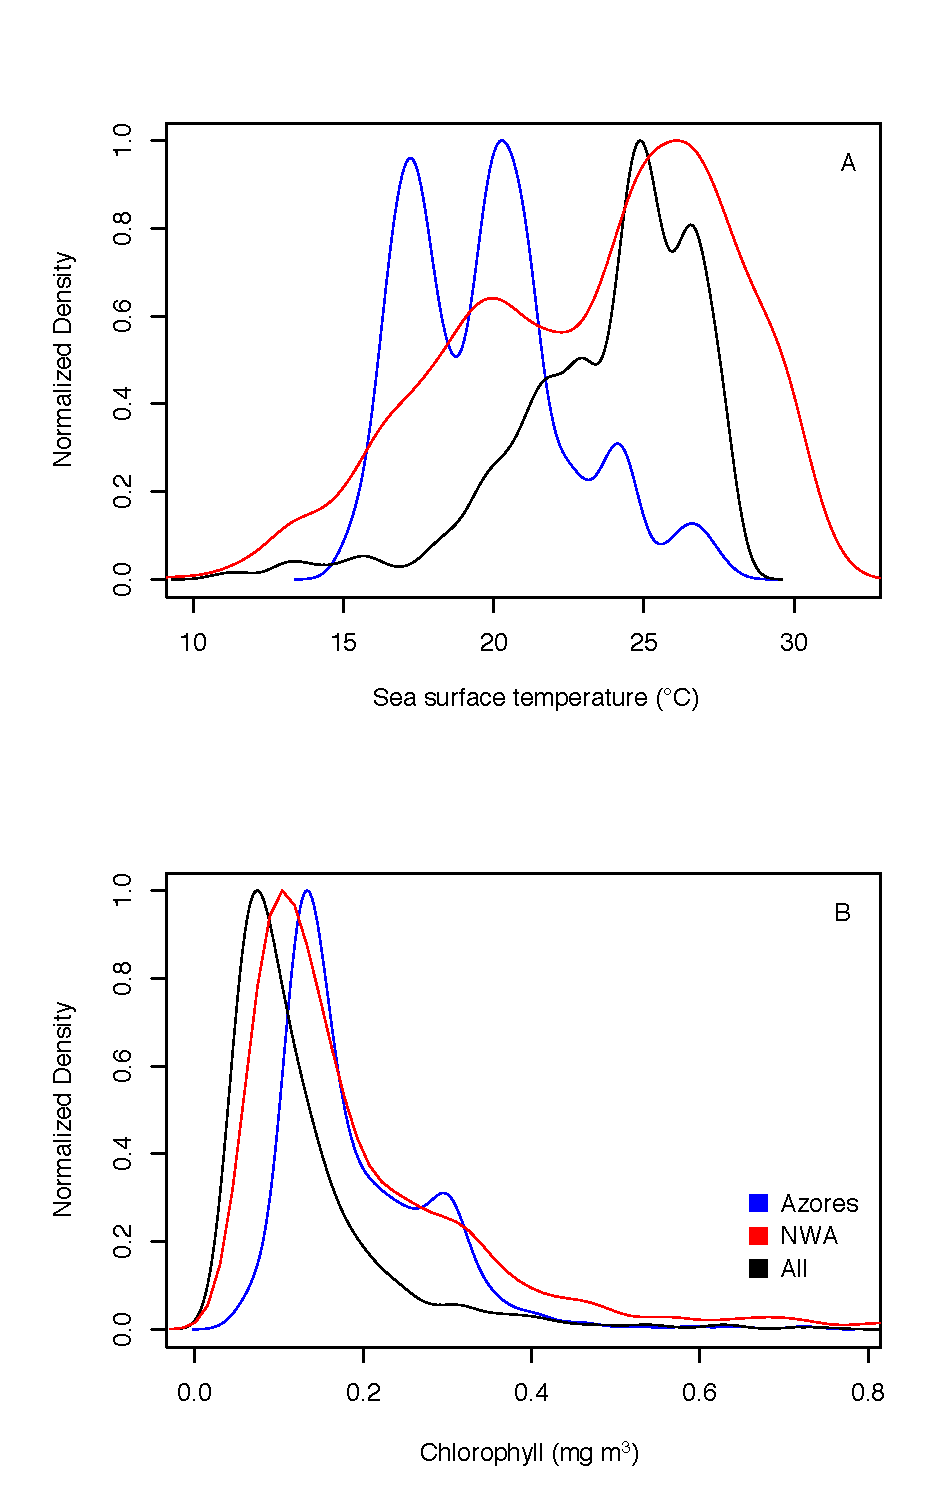
\includegraphics[height=8in, keepaspectratio]{images/A4_FigS5.pdf}
\caption[Distribution of SST and chlorophyll concentrations experienced by satellite and conventional-tagged swordfish in the North Atlantic]{Normalized density distributions of SST (A) and chlorophyll concentrations (B) experienced by satellite-tagged swordfish in the Azores (blue) and northwest Atlantic (red) and a subset of conventional-tagged swordfish in the North Atlantic (black) for which remote-sensing data was available.}
\label{fig:a4f5}
\end{figure}
